\documentclass[citation\_needed]{subfiles}
\begin{document}

L'Annotation Workbench (AWB) est un outil permettant la gestion des annotations, ces dernières pouvant provenir d'un corpus ou être produites par une cartouche. Cela inclut leur création, validation (manuelle ou automatique) sur des corpus de test, visualisation via des concordanciers, comparaison avec d'autres cartouches, etc.
\begin{itemize}
    \item annotation (screenshot "qualify" ?)
    \item évaluation (screenshot "report")
    \item validation (screenshot vue validate) ?
    \item comparer annotations
\end{itemize}

\begin{figure}[ht!]
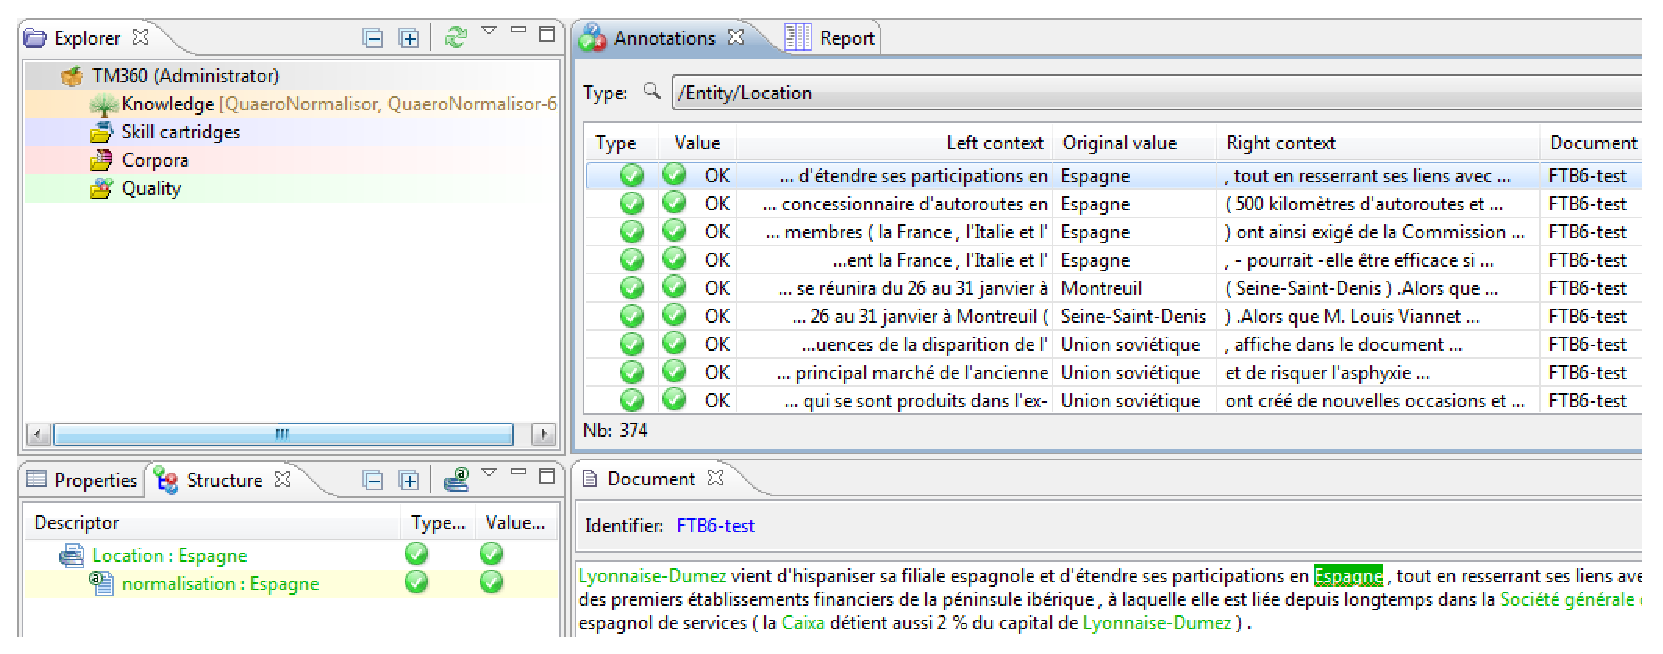
\includegraphics[scale=0.6]{images/Luxid/AWB-1}
\caption{La vue annotation d'AWB}
\label{fig:AWB-overview}
\end{figure}

\end{document}